\section{Learned Elimination Inside Kira's Evolving Matrix}
\label{sec:live-matrix}
The row comparison in Section~\ref{sec:cost-comparison} used fixed
source identities to simplify target expressions before the final Kira
call. To test the intended use inside the solver, we now apply the frozen
row model during Kira's symbolic forward elimination. The input is the
current selected IBP matrix, and every exact row update changes the state
used for the next prediction. Kira continues to generate and select
equations, preserve its integral ordering, normalize the triangular
system and perform back substitution~\cite{Kira3}.

\subsection{Choices in the current IBP matrix}
We retain the matrix notation of Eq.~\eqref{eq:reduction-action}.
At step $n$, $A^{(n)}_{rj}$ is the coefficient of integral $j$ in
identity row $r$.
Let $w(j)$ be Kira's ordering weight for integral column $j$, with larger
weights denoting integrals to eliminate earlier. The leading column of a
nonzero row $r$ and the rows with a common leading column are
\begin{equation}
 h_n(r)=\mathop{\rm arg\,max}_{j:A^{(n)}_{rj}\ne0}w(j),
 \qquad
 R_k^{(n)}=\{r:h_n(r)=k\}.
\end{equation}
At each step we take the largest-weight column that leads at least two
rows. If this column is $k_n$, the allowed choices are
\begin{equation}
 \mathcal A_n=
 \{(q,r,k_n):q,r\in R_{k_n}^{(n)},\ q\ne r\}.
 \label{eq:live-actions}
\end{equation}
Here $q$ is the source row and $r$ is the destination row.
The prescribed master columns remain protected. A proposed elimination
of a protected master, or a zero pivot at the public sampling point,
causes the learned trial to fail its interface check.

The model assigns probabilities to every pair in
Eq.~\eqref{eq:live-actions} and selects the largest score. Kira then uses
its existing symbolic update to calculate
\begin{equation}
 A^{(n+1)}_{rj}
 =A^{(n)}_{rj}
 -\frac{A^{(n)}_{rk_n}}{A^{(n)}_{qk_n}}A^{(n)}_{qj}.
 \label{eq:live-update}
\end{equation}
All these rows represent zero identities, so this operation preserves
their solution space. The new destination row has a lower leading
integral, or becomes zero and leaves the matrix. It can supply a source
row in a later step. The next prediction therefore uses the updated
identities throughout the matrix.

We use the saved 132-feature representation and model weights without
retraining. The family definition, master labels and current rows supply
the features; construction records and reference master coefficients
remain outside the predictions. Rational coefficients at the fixed
public finite-field point supply cancellation features. Kira and Fermat
perform the actual row updates with symbolic rational coefficients.
The process holding the model remains available during one forward
solve, and it receives the initial matrix followed by each changed row.
A system with no allowed row updates does not load the model.

\subsection{Matched controls and measurements}
We use the same seven families with independent master bases and 99 targets as the
native comparison in Section~\ref{sec:cost-comparison}. They include three
one-loop box profiles, a one-loop bubble, triangle and tadpole, and a
two-loop propagator. All methods use the same restricted native seed
bounds, target components, preferred masters and symbolic output checks.

Four methods distinguish the learned choice from changes needed to
measure it. Stock Kira uses the installed solver. Instrumented Kira
retains that solver's forward algorithm and records its exact updates.
The deterministic control uses the largest repeated leading integral
defined above and selects a source by Kira's row-length and integral-order
rule. A stable row identifier selects its destination. The learned
method uses the same serial schedule and selects both rows from the
allowed pairs. This control separates the model's decisions from the
effect of the new schedule. Both methods return the triangular system
to Kira for normalization and back substitution.

Each method runs three times per family on the same node, with rotated
execution order and one computation thread. Complete elapsed time
includes preparation, inference, exact algebra, target combination and
coefficient verification. We also time the forward-elimination phase
directly inside Kira and record model loading separately. The diagnostic
quantity
\begin{equation}
 T_{\mathrm{fwd,load\ excluded}}
 =T_{\mathrm{fwd}}-T_{\mathrm{model\ load}}
\end{equation}
subtracts that recorded loading interval; it retains feature construction,
scoring, communication and exact row updates. It is a timing
decomposition of these runs; a separate run with a preloaded model
has not been measured. Ratios use three-repeat medians and the
paired geometric mean of Eq.~\eqref{eq:cost-ratio}. Forward-stage ratios
include only cases with actual row updates in both methods.
The tadpole batch needs no forward row updates and does not contribute
to those phase ratios.

For each committed update, we retain the convention
$1+2n_q$, where $n_q$ is the source-row nonzero count.
This counts coefficient-field operations and excludes the internal
polynomial work in rational simplification. Elapsed time includes that
work and the candidate trial updates used to prepare features.
The tests keep the action capacity at 10,000, the matrix capacity at
10,000 rows and 250,000 nonzeros, and use bounded time and memory.
These limits bound the systems and action sets tested here.

\subsection{Exact checks and measured results}
All 84 final trials produced the prescribed symbolic master
coefficients. Independent evaluation of the archived native exports
passed 3,564 checks of target coefficients at independent sample
points, and the saved row updates passed
12,708 independent finite-field checks. The model made
1,413 choices across its repeated runs. In 465 choices,
its source row had already changed in an earlier elimination.
These records establish that the model acted on an evolving identity
matrix~\cite{KiraLiveMatrixData}.

The complete elapsed-time ratios for the learned method were
1.305 against stock Kira, 1.286 against instrumented Kira,
and 1.274 against the deterministic control. Within forward
elimination itself, the ratio against instrumented Kira was
276.149 over 6 active family batches. After subtracting the
recorded model-loading interval, the ratio was 62.270.
For those active batches, the native forward-stage medians ranged from
0.003267 to 0.076143 seconds, while the learned medians ranged from
3.061 to 6.909 seconds.

Summing one median operation count per family gives 5,771
coefficient operations for the learned method, 5,070 for
instrumented Kira and 5,097 for the deterministic control.
The corresponding learned and native row-update totals were
471 and 470.
These sums count each family once, while the independent checks above
cover all repeated runs. Figures~\ref{fig:live-times}
and~\ref{fig:live-operations} show the family-level measurements.

\begin{figure}[htbp]
\centering
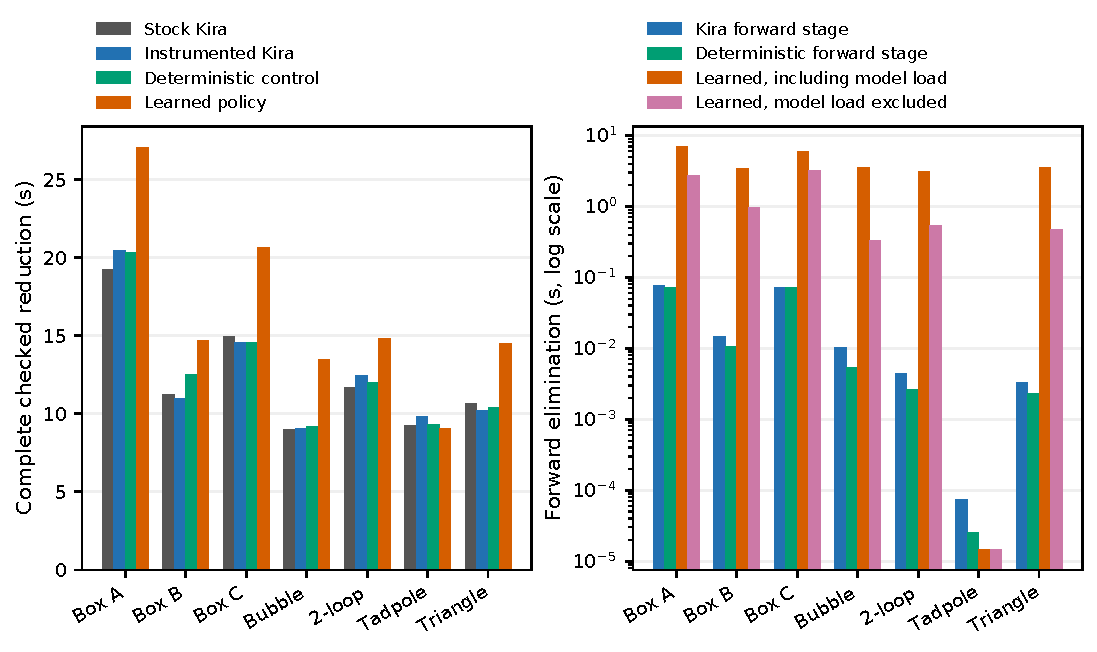
\includegraphics[width=\linewidth]{figures/live_kira_times.pdf}
\caption{Complete checked reduction time and the forward-elimination
time measured inside Kira. Bars show three-repeat medians. The forward
panel uses a logarithmic time axis and separately shows the learned time
after subtracting the recorded model-loading interval. The tadpole
case has no row updates, so its forward time measures phase overhead.
Box A, B and C denote profiles 0173, 0633 and 0156, respectively.}
\label{fig:live-times}
\end{figure}
\begin{figure}[htbp]
\centering
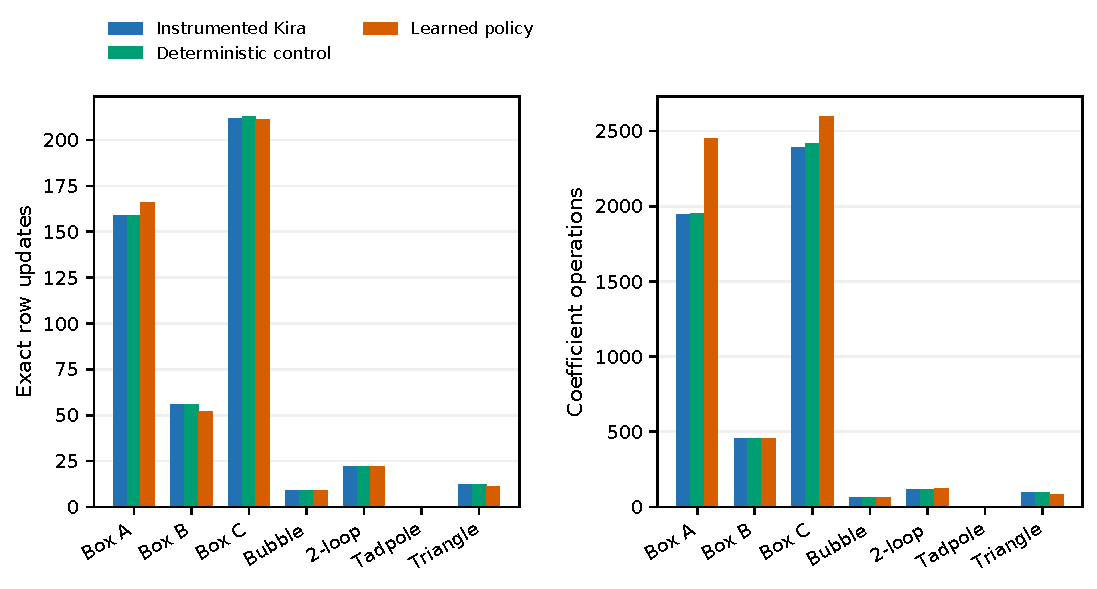
\includegraphics[width=\linewidth]{figures/live_kira_operations.pdf}
\caption{Committed row updates and coefficient-field operations for the
same evolving matrices. Each update contributes $1+2n_q$ operations.
The count excludes candidate scoring and polynomial simplification,
whose costs remain in the time measurements.}
\label{fig:live-operations}
\end{figure}
\FloatBarrier

\subsection{Implications for the proposed reduction policy}
This experiment tests learned choices inside Kira's changing selected
IBP matrix. The measured cost includes the consequences of those choices
for later rows and for the final exact reduction. The current model
increases aggregate runtime, and its summed coefficient-operation count
also exceeds the native count. Excluding model loading does not produce
a forward-elimination speedup in this comparison.

Kira's native forward phase is already short for these selected systems.
The added feature construction and scoring therefore have a small
available time budget. The model was trained on target-row reductions
with fixed source identities, so its application to changing identity
rows also tests transfer beyond those training states. The results apply
to the stated one- and two-loop families and a forward policy that
preserves Kira's integral ordering. Larger independent multiloop systems, other admissible
pivot-column choices and learned back-substitution order remain outside
the present experiment.
